\chapter{Descrizione della soluzione}\label{chp:04-solution}
In questo capitolo è approfondito l'aspetto puramente pratico e le fasi che hanno portato alla realizzazione della soluzione; 
inoltre vengono mostrate le applicazioni pratiche degli aspetti teorici enunciati nei capitoli precedenti.
%
\vspace{1.5 cm}
\hfill\break
% BREVE DESCRIZIONE DELLA SOLUZIONE
La soluzione proposta in questa testi implementa un servizio di API REST, che si appoggia a un database Postgres, accessibile 
attraverso apposite URL; questo servizio permette di effettuare richieste al sistema di raccomandazione e di effettuare degli 
aggiornamenti a questa base di dati.
%
\section*{Preparazione della base di dati}
Prima di poter costruire il sistema di raccomandazione proposto in questa tesi, sono state eseguite delle operazioni preliminari 
per poter impostare il progetto di Django e la relativa applicazione che implementerà effettivamente la soluzione. 
% TASSONOMIE E DATABASE CON I MODELS (package MPTT)
Come descritto nei capitoli precedenti per procedere alla costruzione di un sistema di raccomandazione bisogna avere a disposizione 
una base di dati solida da cui attingere tutte le informazioni; ed è proprio questo il primo passo che è stato seguito, disegnare 
e progettare un database da cui partire per la realizzazione degli algoritmi proposti.
In generale Moon Cloud possiede una struttura delle Evaluation e dei Control ad albero, di conseguenza anche le tabelle del database 
rispecchiano questa struttura, partendo dalle considerazioni fatte sulle tecniche descritte nei capitoli precedenti si è deciso, che 
per implementare un database relazionale che gestisse dati gerarchici, di utilizzare la tecnica
definita come \textit{Modified Preorder Tree Traversal Algorithm}, la quale permette di massimizzare l'efficienza nelle 
operazioni di recupero dei dati, e quindi velocizzare i processi di raccomandazione, ma scendendo a compromessi per quanto riguarda le 
operazioni d'inserimento e spostamento dei nodi all'interno della struttura. 
Il package MPTT è una app di Django che ha come obiettivo quello di semplificare il più possibile la realizzazione dei Model, utilizzati 
per la generazione della base di dati, e la gestione della struttura di dati ad albero; si prende cura di tutti i dettagli riguardanti la 
realizzazione delle tabelle e dei campi \textit{left} e \textit{right} associati ad ogni nodo della tassonomia, mettendo a disposizione dei 
tool per poter lavorare con le istanze dei Model. Nel Listing \ref{lst:model} è possibile trovare le porzioni principali del 
codice costituenti i Model.
%
% MODELS CODES
\lstset{style=python_code_style}
\begin{lstlisting}[language=Python, label=lst:model, caption={Parti principali del codice che costituiscono i Model della soluzione.}]
# TARGET TYPE MODEL
 
class TargetType(models.Model):
    """
    Target supported by Moon Cloud system
    """
    TYPES = (
        ('host', 'host'),
        ('windows', 'windows'),
        ('url', 'url'),
        ('azure', 'azure'),
        ('aws', 'aws')
    )
    name = models.CharField(max_length=150, choices=TYPES, default="host")
    descr = models.TextField(max_length=1000, default="none")  # Description of a target
 
    def __str__(self):
        return str(self.name)
 
    class Meta:
        ordering = ['id']
 
 
# CONTROL MODEL
 
class Control(MPTTModel):
    """
    Controls that can be part of Evaluations
    """
    other_id = models.IntegerField(default=-1, unique=True)
    parent = TreeForeignKey('self', on_delete=models.CASCADE, null=True, blank=True, related_name='children')
    name = models.CharField(max_length=150, unique=True)
    descr = models.TextField(max_length=1000, default="none")  # Description of a node in the taxonomy
    TYPES = (
        ('cat', 'category'),
        ('con', 'control')
    )
    # Possible node type of the taxonomy (category node or control node)
    node_type = models.CharField(max_length=3, choices=TYPES, default='cat')
    target_type = models.ForeignKey(TargetType, blank=True, null=True, on_delete=models.CASCADE)  # It's null for the root node and category nodes
 
    def __str__(self):
        return str(self.name)
 
    class MPTTMeta:
        level_attr = 'level'
        order_insertion_by = ['name']
 
    class Meta:
        ordering = ['tree_id', 'lft']
 
 
# EVALUATION MODEL
 
class Evaluation(MPTTModel):
    """
    Evaluation is composed by one or more Controls, and can be used by Users
    """
    other_id = models.IntegerField(default=-1, unique=True)
    parent = TreeForeignKey('self', on_delete=models.CASCADE, null=True, blank=True, related_name='children')
    name = models.CharField(max_length=150, unique=True)
    descr = models.TextField(max_length=1000, default="none")  # Description of a node in the taxonomy
    TYPES = (
        ('cat', 'category'),
        ('eva', 'evaluation')
    )
    # Possible node types of the taxonomy (category node or evaluation node)
    node_type = models.CharField(max_length=3, choices=TYPES, default='cat')
    controls = models.ManyToManyField(Control)  # Evaluation can be composed of one or more controls
 
    def __str__(self):
        return str(self.name)
 
    class MPTTMeta:
        level_attr = 'level'
        order_insertion_by = ['name']
 
    class Meta:
        ordering = ['tree_id', 'lft']
 
 
# USER MODEL
 
class User(models.Model):
    """
    User registered to Moon Cloud with an email address, and can insert Target and launch Evaluations
    """
    other_id = models.IntegerField(default=-1, unique=True)
    email = models.EmailField(max_length=50, unique=True)
    evaluations = models.ManyToManyField(Evaluation, blank=True)  # Evaluations chosen by user
 
    def __str__(self):
        return str(self.email)
 
    class Meta:
        ordering = ['other_id', 'id']
 
 
# TARGET MODEL
 
class Target(models.Model):
    """
    Target (can be more than one) chosen by the user
    """
    user = models.ForeignKey(User, on_delete=models.CASCADE)  # User has chosen a target_type
    other_id = models.IntegerField(default=-1, unique=True)
    target_type = models.ForeignKey(TargetType, on_delete=models.CASCADE)  # TargetType Id
 
    def __str__(self):
        return str(self.user) + " " + str(self.other_id) + " " + str(self.target_type)
 
    class Meta:
        ordering = ['user']
\end{lstlisting}
%
A partire da questi Model vennero introdotte nel database le seguenti tabelle, le quali è possibile visionare nella Figura 
\ref{fig:str_db_project}.
\begin{description}
    \item[Control:] contiene l'insieme dei software, o soltanto i riferimenti, che vengono poi effettivamente eseguiti all'interno 
    di una Evaluation, i campi \texttt{other\_id} (identificativo dell'Evaluation che fa riferimento al database effettivo di Moon Cloud), 
    descr (una descrizione del funzionamento del controllo), \texttt{node\_type} (definisce se il nodo è un Evaluation o una Categoria) 
    definiscono le caratteristiche del controllo mentre lft, rght, \texttt{tree\_id}, \texttt{level} e \texttt{parent} sono introdotti 
    automaticamente dal package MPTT per poter rappresentare i dati in modo gerarchico, infine \texttt{target\_type\_id} rappresenta, quel 
    controllo a quale Target viene associato.
    \item[Evaluation:] contiene l'insieme di Evaluation che un utente può eseguire per un certo Target, e allo stesso modo 
    i campi contenuti nella tabella Control. La tabella intermedia \textit{evaluation\_controls}permette di memorizzare quali Controlli 
    sono associati a quali Evaluation.
    \item[User:] contiene gli utenti registrati alla piattaforma Moon Cloud, e sono anche loro, come con le tabelle precedenti, 
    identificati con un campo \texttt{other\_id}, e distinti da un email. La tabella intermedia \textit{user\_evaluations} permette di memorizzare 
    quali Evaluation un utente ha selezionato e usato.
    \item[Target:] contiene i  Target (o asset) un utente ha inserito e sui quali vuole effettuare dei processi 
    di monitoraggio e verifica, attraverso l'applicazione di politiche e Evaluation.
    \item[TargetType:] contiene i tipi di Target supportati da Moon Cloud. In generale sono supportati: \textit{URL}, 
    rappresentante l'URL dell'applicativo web, \textit{Host}, viene specificato l'indirizzo IP identificativo di un host e si distingue 
    tra sistema operativo \textit{Windows} o \textit{Linux} eseguito su esso, \textit{Aws}, rappresentante il servizio di cloud computing del 
    gruppo Amazon, e \textit{Azure}, definisce un servizio cloud fornito da Microsoft.
\end{description}
%
\begin{figure}[ht!]
    \centering
    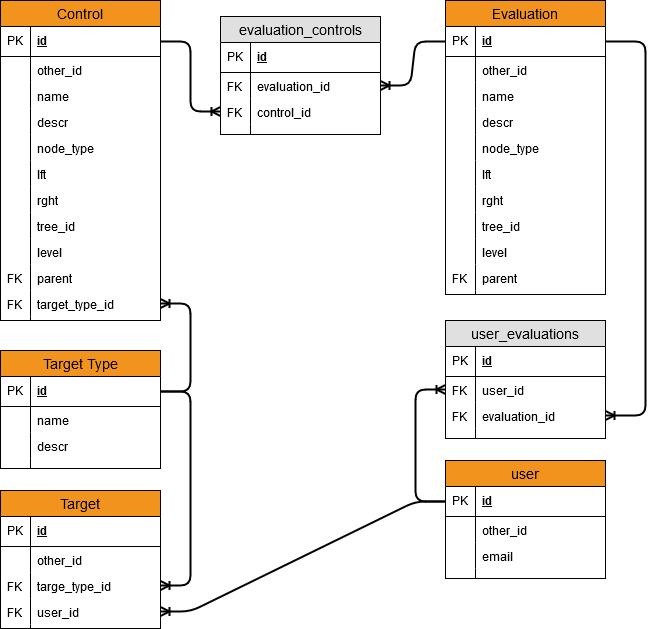
\includegraphics[scale=0.6]{images/MoonCloudRecommendation_ER.png}
    \caption{Struttura del database.}
    \label{fig:str_db_project}
\end{figure}
%
\newpage
%
% VIEW A SCOPO DIDATTICO
%\hfill\break
\section*{Realizzazione delle View}
Successivamente per poter testare che la tassonomia creata per le Evalution e i Controlli fosse corretta e funzionante si è 
implementata un'interfaccia Web a scopo didattico.
Avviando il server, viene mostrata una home page la quale contiene una barra di navigazione da cui è possibile accedere,
attraverso il \textit{Admin}, alla admin page offerta da Django (successivamente personalizzata, per poter manipolare la base di dati, 
e aggiungere, eliminare item o utenti), mentre tramite il link \textit{Home} è possibile tornare a 
questa pagina. Il contenuto di questa pagina mostra una breve descrizione di un sistema di raccomandazione, e accedere tramite i due 
appositi pulsanti alle pagine specifiche per la navigazione della tassonomia delle Evaluation piuttosto che dei Controlli; tutto questo 
viene mostrato dalla Figura \ref{fig:MCRS_homepage} e il relativo Listing \ref{lst:view_homepage}.
%
\begin{figure}[ht!]
    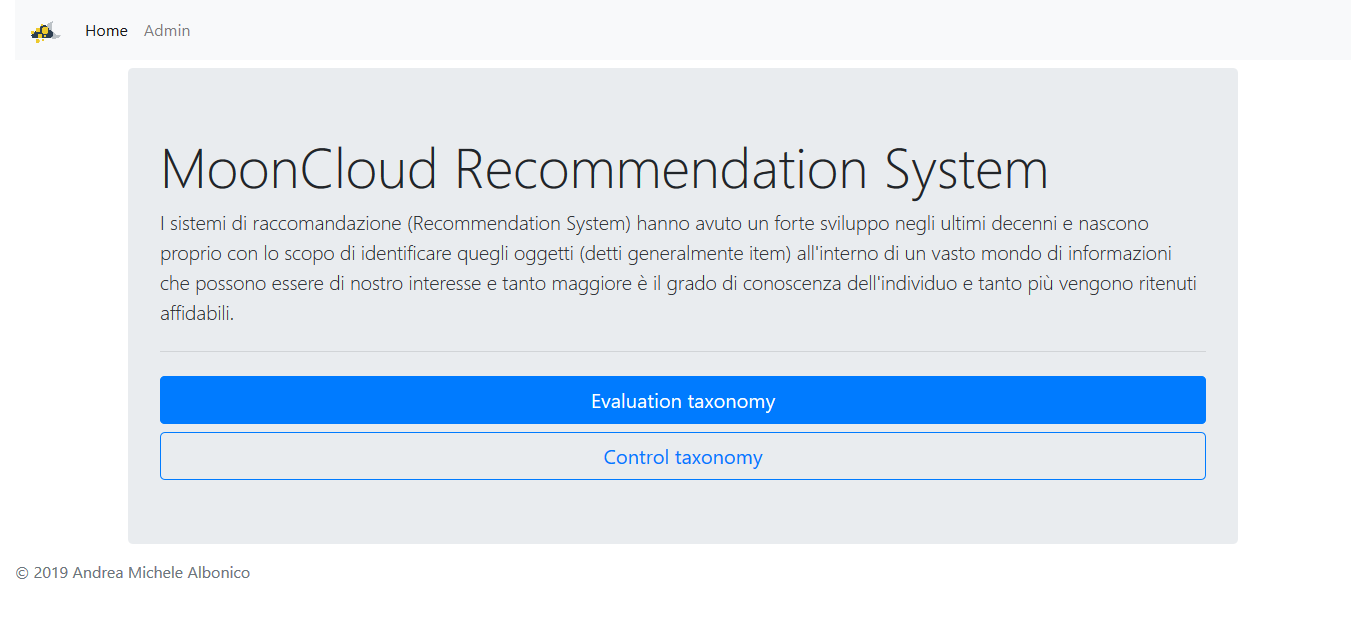
\includegraphics[scale=0.3]{images/MCRS_homepage.png}
    \caption{Home page dell'applicativo web a scopo didattico.}
    \label{fig:MCRS_homepage}
\end{figure}
\lstset{style=python_code_style}
\begin{lstlisting}[language=Python, label=lst:view_homepage, caption={Parte principale del codice delle View della soluzione per gestire l'accesso 
    alla home page.}]
def index(request):
    """
    Index page where you can choose to navigate the evaluation taxonomy or the control taxonomy.
    :param request: HTTP request
    :return: HTTP response with the template to show to the user
    """
    return render(request, "recommendation_app/index.html")
\end{lstlisting}
%
Una volta scelta la tassonomia, di Controlli o delle Evaluation, su cui si vuole navigare, viene mostrata una pagina dove nella metà a sinistra 
troviamo la possibilità di selezionare un nodo della tassonomia e l'operazione che si vuole svolgere su quel nodo, inoltre, è possibile effettuare 
una richiesta di generazione di file in formato e linguaggio DOT e relativa immagine in formato .png, attraverso il pulsante \textit{Request schema}. 
Proseguendo più in basso, vengono mostrati tutti i nodi a cui è stato associato il tipo Categoria e il tipo Evaluation. Nella porzione destra della 
pagina web viene mostrata l'intera struttura della tassonomia e un link da quale è possibile accedere a una pagina di dettaglio che mostra una 
simile a quella presente sul database. Questa pagine è visibile dalla Figura \ref{fig:MCRS_taxindex} e dal Listing \ref{lst:view_tax_homepage}.\hfill\break
%
\begin{figure}[ht!]
    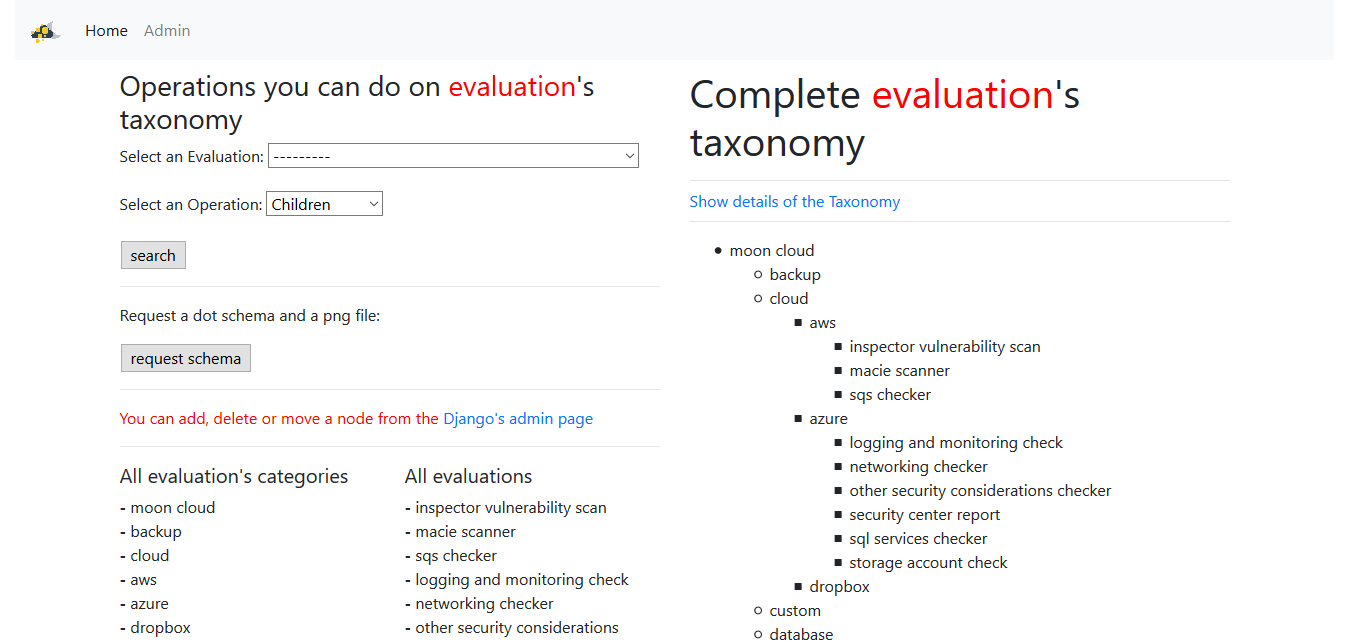
\includegraphics[scale=0.3]{images/MCRS_taxindex.png}
    \caption{Home page per la navigazione della tassonomia delle Evaluation.}
    \label{fig:MCRS_taxindex}
\end{figure}
%
\lstset{style=python_code_style}
\begin{lstlisting}[language=Python, label=lst:view_tax_homepage, caption={Home page dalla quale è possibile richiamare 
    diverse operazioni eseguibili sulla tassonomia.}]
def tax_index(request, taxonomy_used):
    """
    The home page shows all taxonomy and a form to make operations on it.
    :param request: HTTP request
    :param taxonomy_used: specify if it's used the Control taxonomy or the Evaluation taxonomy
    :return: HTTP response with the template to show to the user
    """
    # If this is a POST request we need to process the form data
    if request.method == 'POST':
        # Create a form instance and populate it with data from depending on the taxonomy_used
        if (taxonomy_used == "evaluation"):
            form = EvaluationOperationForm(request.POST)
        else:
            form = ControlEvaluationForm(request.POST)
        # Check whether it's valid:
        if form.is_valid():
            # Process the data in form.cleaned_data as required
            nodename_form = form.cleaned_data['nodeName']
            taxonomy_operation_form = form.cleaned_data['actionTax']
            # Redirect to a new URL (page that show a part of the taxonomy, depending on the action user has chosen):
            return redirect(
                reverse('rec:tax_index', args=[taxonomy_used]) + str(nodename_form) + '_' + taxonomy_operation_form)
    # If id's a GET method we'll create a blank form
    else:
        if (taxonomy_used == "evaluation"):
            form = EvaluationOperationForm()
        else:
            form = ControlEvaluationForm()
 
    # Depending on the taxonomy_used, I'm getting all the categories of Evaluations or Controls taxonomy and save it in a
    # list called "categories_list"
    if (taxonomy_used == "evaluation"):
        q_categories = Evaluation.objects.filter(node_type='cat')
    else:
        q_categories = Control.objects.filter(node_type='cat')
    categories_list = []
    for node in q_categories:
        categories_list.append(node.name)
 
    # Depending on the taxonomy_used, I'm getting all the categories of Evaluations or Controls node in the taxonomy
    # and save it in a list called "node_list"
    if (taxonomy_used == "evaluation"):
        q_nodes = Evaluation.objects.filter(node_type='eva')
    else:
        q_nodes = Control.objects.filter(node_type='con')
    node_list = []
    for node in q_nodes:
        node_list.append(node.name)
 
    # Depending on the taxonomy_used, I'm getting all the Evaluations or Controls taxonomy
    if (taxonomy_used == "evaluation"):
        tax = Evaluation.objects.all()
    else:
        tax = Control.objects.all()
 
    # Passing the complete taxonomy and data to fill the form so you can operate on the taxonomy
    args = {'tax': tax,
            'categories': categories_list,
            'nodes': node_list,
            'form': form,
            'request_path': taxonomy_used}
 
    return render(request, "recommendation_app/tax_index.html", args)
\end{lstlisting}
%
Le attività che è possibile svolgere sulla tassonomia, sia dei Controlli sia delle Evaluation, sono le seguenti, mentre le operazioni 
di manipolazione dei dati memorizzati dal database vengono svolte con l'ausilio della admin page messa a disposizione da Django.\hfill\break
\begin{itemize}
    \item Per ogni singolo nodo è possibile recuperare: i discendenti, i figli, la famiglia o i fratelli. Si ottiene un risultato come nella 
    Figura \ref{fig:MCRS_taxnodedetails} nel caso in cui si è scelti l'\textit{Evaluation Http robustness check} e si vuole ritornare tutta la 
    famiglia di quel nodo.
    %
    \begin{figure}[ht!]
        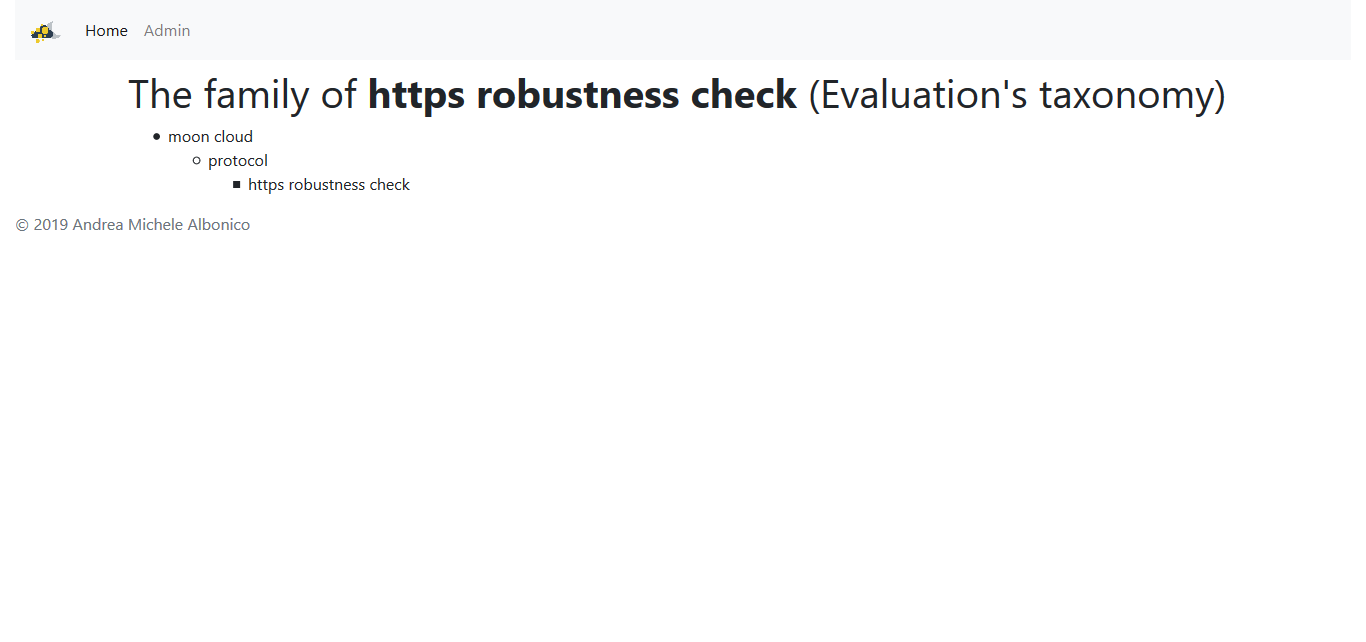
\includegraphics[scale=0.3]{images/MCRS_taxnodedetails.png}
        \caption{Risultato dell'operazione selezionata sul nodo in questione.}
        \label{fig:MCRS_taxnodedetails}
    \end{figure}
    %
    \lstset{style=python_code_style}
    \begin{lstlisting}[language=Python, label=lst:view_tax_nodedetails, caption={Codice utilizzato all'interno delle View per 
        implementare le operazioni per restituire i discendenti, i figli, la famiglia o i fratelli.}]
    # Methods to navigate the taxonomy
 
    def show_descendants(request, nodename, taxonomy_used):
        """
        Based on the MPTT's method 'get descendants' that return the descendants of a model instance, in tree order
        :param request: HTTP request
        :param nodename: name (it's unique for each node) of a node in the taxonomy
        :param taxonomy_used: specify if it's used the Control taxonomy or the Evaluation taxonomy
        :return: HTTP response with the template to show to the user
        """
        if (taxonomy_used == 'evaluation'):
            q_result = Evaluation.objects.get(name=nodename).get_descendants(include_self=False)
            # Get the count of descendants of the model instance
            q_result_num = Evaluation.objects.get(name=nodename).get_descendant_count()
        else:
            q_result = Control.objects.get(name=nodename).get_descendants(include_self=False)
            # Get the count of descendants of the model instance
            q_result_num = Control.objects.get(name=nodename).get_descendant_count()
 
        return render(request, "recommendation_app/tax_node_details.html",
                    {'tax_type': (str(taxonomy_used)).capitalize(),
                    'descendants': q_result,
                    'node_exe': nodename,
                    'method': 'descendants',
                    'num_descendants': q_result_num})
 
 
    def show_children(request, nodename, taxonomy_used):
        """
        Based on the MPTT's method 'get children' that return the immediate children of a model instance, in tree order
        :param request: HTTP request
        :param nodename: name (it's unique for each node) of a node in the taxonomy
        :param taxonomy_used: specify if it's used the Control taxonomy or the Evaluation taxonomy
        :return: HTTP response with the template to show to the user
        """
        if (taxonomy_used == 'evaluation'):
            q_result = Evaluation.objects.get(name=nodename).get_children()
        else:
            q_result = Control.objects.get(name=nodename).get_children()
 
        return render(request, "recommendation_app/tax_node_details.html",
                    {'tax_type': (str(taxonomy_used)).capitalize(),
                    'children': q_result,
                    'node_exe': nodename,
                    'method': 'children'})
 
 
    def show_family(request, nodename, taxonomy_used):
        """
        Based on the MPTT's method 'get family' that return the ancestors, the model instance itself and the descendants,
        in tree order
        :param request: HTTP request
        :param nodename: name (it's unique for each node) of a node in the taxonomy
        :param taxonomy_used: specify if it's used the Control taxonomy or the Evaluation taxonomy
        :return: HTTP response with the template to show to the user
        """
        if (taxonomy_used == 'evaluation'):
            q_result = Evaluation.objects.get(name=nodename).get_family()
        else:
            q_result = Control.objects.get(name=nodename).get_family()
 
        return render(request, "recommendation_app/tax_node_details.html",
                    {'tax_type': (str(taxonomy_used)).capitalize(),
                    'family': q_result,
                    'node_exe': nodename,
                    'method': 'family'})
 
 
    def show_siblings(request, nodename, taxonomy_used):
        """
        Based on the MPTT's method 'get siblings' that return siblings of the model instance (root nodes are considered
        to be siblings of other root nodes)
        :param request: HTTP request
        :param nodename: name (it's unique for each node) of a node in the taxonomy
        :param taxonomy_used: specify if it's used the Control taxonomy or the Evaluation taxonomy
        :return: HTTP response with the template to show to the user
        """
        if (taxonomy_used == 'evaluation'):
            q_result = Evaluation.objects.get(name=nodename).get_siblings()
        else:
            q_result = Control.objects.get(name=nodename).get_siblings()
 
        return render(request, "recommendation_app/tax_node_details.html",
                    {'tax_type': (str(taxonomy_used)).capitalize(),
                    'siblings': q_result,
                    'node_exe': nodename,
                    'method': 'siblings'})
    \end{lstlisting}
    \item Attraverso il pulsante \textit{request schema} nella home page della tassonomia si può effettuare una richiesta al software 
    Graphviz il quale attraverso un file scritto in linguaggio DOT genera lo schema della tassonomia sotto forma d'immagine in formato .png.\hfill\break
    Il DOT è un linguaggio descrittivo per grafi, tipicamente i file hanno estensione .gv o .dot, che in combinazione con il software Graphviz è possibile 
    effettuare il rendering della sintassi DOT in un immagine più significativa. Un esempio di tale linguaggio è mostrato nel Listing \ref{lst:DOT_eval} 
    viene mostrato un esempio di scrittura con linguaggio DOT.
    \lstset{style=python_code_style}
    \begin{lstlisting}[language=Python, label=lst:DOT_eval, caption={Codice parziale utilizzato per realizzare lo schema della tassonomia
        per le Evaluation.}]
    graph {
        1 [label="moon cloud"]
        12 [label="protocol"]
        1 -- 12
        11 [label="infrastructure"]
        1 -- 11
        4 [label="cloud"]
        1 -- 4
        16 [label="backup"]
        1 -- 16
        2 [label="database"]
        1 -- 2
        13 [label="web"]
        1 -- 13
        9 [label="human"]
        1 -- 9
        8 [label="custom"]
        1 -- 8
        3 [label="operating system"]
    }
    \end{lstlisting}
    %
    \lstset{style=python_code_style}
    \begin{lstlisting}[language=Python, label=lst:view_DOT_eval, caption={Codice utilizzato per la realizzazione del
        file .dot e relativa immagine .png.}]
    def dot_graph(request, taxonomy_used):
        """
        Create the .dot file (based on the Dot language) and the graph showing the taxonomy in .png format
        :param request: HTTP request
        :param taxonomy_used: specify if it's used the Control taxonomy or the Evaluation taxonomy
        :return: HTTP response with the template to show to the user
        """
        # Create a graph object
        taxonomy_dot_object = Graph(comment='Taxonomy', format='png')
        # Fill the graph with every node in the database (evaluations/controls node and categories nodes), 
        # and create a link with the parent node
        if (taxonomy_used == 'evaluation'):
            taxonomy_nodes = Evaluation.objects.all()
        else:
            taxonomy_nodes = Control.objects.all()
        i = 0
        for node in taxonomy_nodes.order_by('level'):
            # This If construct will prevent the adding of an empty node to the root node in the graph
            if (i == 0):
                # Insert the root node
                taxonomy_dot_object.node(str(node.id), label=str(node.name))
            else:
                # Insert the other nodes
                taxonomy_dot_object.node(str(node.id), label=str(node.name))
                taxonomy_dot_object.edge(str(node.parent_id), str(node.id))
            i += 1
        # Specify where I want to save the .png image and the .dot file
        taxonomy_dot_object.render('taxonomy_output/taxonomy.dot')
 
        # This function is used to zip a directory
        def make_zipdir(path, ziph):
            # Ziph is zipfile handle
            for root, dirs, files in os.walk(path):
                for file in files:
                    ziph.write(os.path.join(root, file))
 
        # Making the zip file
        zip_file = zipfile.ZipFile('taxonomy_output.zip', 'w', compression=zipfile.ZIP_DEFLATED)
        make_zipdir('taxonomy_output/', zip_file)
        zip_file.close()
 
        # Remove the directory which was zipped and all files inside
        shutil.rmtree("taxonomy_output/")
 
        return redirect(reverse('rec:index'))
    \end{lstlisting}
    \item Inoltre è possibile osservare in maniera più approfondita le informazioni rilevanti sulla tassonomia contenute nelle 
    tabelle del database; e nel caso, della tassonomia delle Evaluation, è possibile simulare il processo di Item Recommendation, 
    premendo il relativo tasto rispetto al nodo su cui si vuole determinare le altre Evaluation simili.
    %
    \begin{figure}[ht!]
        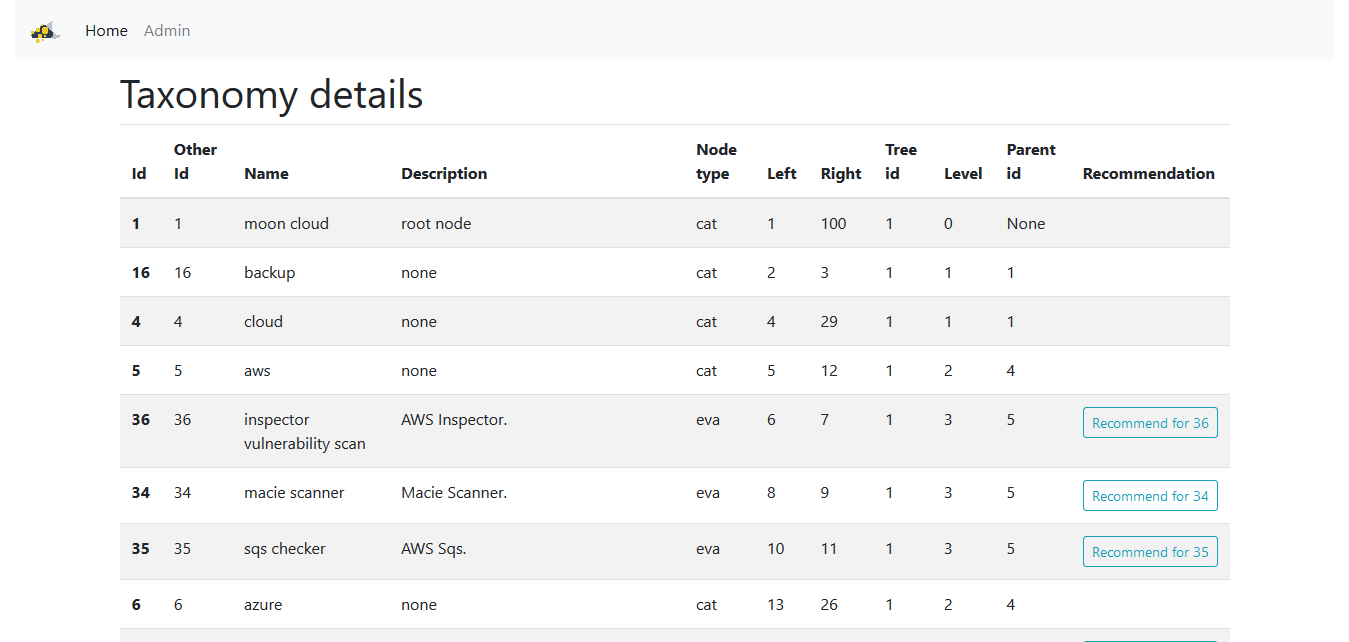
\includegraphics[scale=0.3]{images/MCRS_taxdetails.png}
        \caption{Dettagli della tassonomia sotto forma di tabella come nella base di dati.}
        \label{fig:MCRS_taxdetails}
    \end{figure}
    %
    \lstset{style=python_code_style}
    \begin{lstlisting}[language=Python, label=lst:view_taxdetails, caption={Codice utilizzato per la realizzazione della View che 
        implementa la pagina web del dettaglio della Tassonomia.}]
    def tax_details(request, taxonomy_used):
        """
        Show the taxonomy's details page showing an overview of the taxonomy
        :param request: HTTP request
        :param taxonomy_used: specify if it's used the Control taxonomy or the Evaluation taxonomy
        :return: HTTP response with the template to show to the user
        """
        if (taxonomy_used == 'evaluation'):
            tax_details_obj = Evaluation.objects.all()
        else:
            tax_details_obj = Control.objects.all()
 
        return render(request, "recommendation_app/tax_details.html",
                    {'tax_details': tax_details_obj,
                    'taxonomy_used': taxonomy_used})
    \end{lstlisting}
\end{itemize}
%
\newpage
%
% VIEW PER LE RACCOMANDAZIONI
\section*{View per i processi di raccomandazione}
% visto che il codice l'ho messo nel capitolo precedente, posso mettere qui degli esempi e mostrare le url per richiamare
% questi algoritmi, e nel caso dello User e Item algortihm, mostrare le view che li implementano come REST API 
% (non mostro quella dell'hybrid perché già presente al completo nel capitolo precedente)
In generale gli algoritmi di raccomandazione implementati in questo progetto, e descritti nel Capitolo \ref{chp:03-recommendationSystems}, 
vengono richiamati e utilizzati come API REST, un tipo di architettura basata sul protocollo HTTP. Un sistema REST, per funzionare, prevede 
una struttura degli URL ben definita (atta a identificare univocamente una risorsa o un insieme di risorse) l'utilizzo dei verbi HTTP specifici 
per il recupero d'informazioni (GET), per la modifica (POST, PUT, PATCH, DELETE) e per altri scopi (OPTIONS, ecc.).\hfill\break
In questo caso a ogni URL è associata una azione particolare la quale va a richiamare la View che permette di determinare un insieme di 
raccomandazioni sulla base di un parametro in ingresso, come è mostrato nel Listing \ref{lst:URL_rec}.\hfill\break
\lstset{style=python_code_style}
\begin{lstlisting}[language=Python, label=lst:URL_rec, caption={Porzione parziale del codice contenuto nell'URL mapper per implementare 
    i sistemi di raccomandazione.}]
# RECOMMENDATION VIEWS
 
# Item recommendation process
# Depending on the <str:item_other_id> value I decide on which evaluation of the taxonomy I want to recommend on
path('recommendation/item/<str:item_other_id>/', recommendation_views.item_recommendation,
        name='item_recommendation'),
 
# User recommendation process
# Depending on the <str:user_other_id> value I decide on which user I want to recommend on
path('recommendation/user/<str:user_other_id>/', recommendation_views.user_recommendation,
        name='user_recommendation'),
 
# Hybrid recommendation process (User and Item recommendation process)
# Depending on the <str:User_other_id> value I decide on which user I want to recommend on with an hybrid approach
path('recommendation/hybrid/<str:user_other_id>/', recommendation_views.hybrid_recommendation,
        name='hybrid_ui_recommendation'),
 
# Target recommendation process
# Depending on the <str:target_type_id> value I decide on which user I want to recommend on
path('recommendation/target/<str:target_type_id>/', recommendation_views.target_recommendation,
        name='target_recommendation'),
\end{lstlisting}
Sulla base dell'URL che viene richiamato e sul parametro (come \texttt{user\_other\_id}, \texttt{item\_other\_id}, ecc.) verranno fornite le 
relative raccomandazioni. Nel caso di questo progetto, le View che possono essere richiamate permettono soltanto chiamate HTTP con metodo GET 
e restituiscono una risposta HTTP in formato JSON, queste risposte contengono una lista di dizionari e ciascuno contiene l'\texttt{other\_id} della Evaluation 
che si vuole raccomandare. Di seguito nel Listing \ref{lst:view_rec} vengono mostrati le porzioni di codice rappresentanti 
le View per gli algoritmi di raccomandazione per Item (in questo caso Evaluaiton), Utenti e Target. Inoltre nel Listing \ref{lst:view_rec_ex} è 
possibile osservare alcuni esempi e risposte di richieste HTTP a questi algortmi.\hfill\break
\lstset{style=python_code_style}
\begin{lstlisting}[language=Python, label=lst:view_rec, caption={Porzione parziale del codice contenuto nelle View per implementare
    i sistemi di raccomandazione.}]
# Item recommendation API REST
@api_view(['GET'])
def item_recommendation(request, item_other_id):
    """
    Returns recommendations for the using an item-based recommendation algorithm for the Evaluation `item_other_id`
 
    :param request: http GET request
    :param item_other_id: value representing the other_id of an Item (Evaluation)
    :return: json response with the evaluations to recommend
    """
    # Trying to retrieve the actual node with item_other_id
    item = Evaluation.objects.get(other_id=item_other_id)
 
    similar_item_evaluations = item_recommendation_alg(item_other_id)
    # Cleaning the data, deleting all the keys except 'other_id'
    similar_item_evaluations_serilized = EvaluationSerializerRecommendation(similar_item_evaluations, many=True).data
 
    return JsonResponse(similar_item_evaluations_serilized, safe=False)
 
# User recommendation API REST
@api_view(['GET'])
def user_recommendation(request, user_other_id):
    """
    Returns recommendations for the using an user-based recommendation algorithm for the user `user_other_id`
 
    :param request: http GET request
    :param user_other_id: value representing the other_id of a User
    :return: json response with the evaluations to recommend
    """
    # Trying to retrieve the actual User with user_other_id
    user = User.objects.get(other_id=user_other_id)
 
    target_user_evaluations, similar_user_evaluations = user_recommendation_alg(user_other_id)
    # Cleaning the data, deleting all the keys except 'other_id'
    similar_user_evaluations_serilized = EvaluationSerializerRecommendation(similar_user_evaluations, many=True).data
 
    return JsonResponse(similar_user_evaluations_serilized, safe=False)
 
# Target Recommendation API REST
@api_view(['GET'])
def target_recommendation(request, target_type_id):
    """
    For a target (Target_Type like 'host', 'aws', 'url', etc.) chose by a user this algorithm search the possible
    evaluations that can be recommended for that user.
 
    :param request: http GET request
    :param target_type_id: identifier of a particular target_type
    :return: json response with the evaluations to recommend
    """
    # Trying to retrieve the actual Target Type, with id equal to target_type_id, chosed by a user
    target = TargetType.objects.get(id=target_type_id)
 
    target_evaluations = target_recommendation_alg(target_type_id)
 
    return JsonResponse(target_evaluations, safe=False)
\end{lstlisting}
\lstset{style=python_code_style}
\begin{lstlisting}[language=Python, label=lst:view_rec_ex, caption={Esempi di chiamate e risposte HTTP per i diversi algoritmi di raccomandazione.}]
Esempio di chiamata per lo Item Recommendation Algorithm
URL: http://127.0.0.1:8000/recommendation/item/34/ 
HTTP method: GET
 
Esempio di risposta per lo Item Recommendation Algorithm
HTTP Status: 200 OK
HTTP Response Body:
[
    {"other_id": 35},
    {"other_id": 36}
]
 
Esempio di chiamata per lo User Recommendation Algorithm
URL: http://127.0.0.1:8000/recommendation/user/10/ 
HTTP method: GET
 
Esempio di risposta per lo User Recommendation Algorithm
HTTP Status: 200 OK
HTTP Response Body:
[
    {"other_id": 36}
]
 
Esempio di chiamata per lo Hybrid Recommendation Algorithm
URL: http://127.0.0.1:8000/recommendation/hybrid/10/ 
HTTP method: GET
 
Esempio di risposta per lo Hybrid Recommendation Algorithm
HTTP Status: 200 OK
HTTP Response Body:
[
    {"other_id": 23},
    {"other_id": 24},
    {"other_id": 25},
    {"other_id": 26},
    {"other_id": 28},
    {"other_id": 29},
    {"other_id": 30},
    {"other_id": 31},
    {"other_id": 32},
    {"other_id": 35},
    {"other_id": 36},
    {"other_id": 43},
    {"other_id": 45},
    {"other_id": 46},
    {"other_id": 47},
    {"other_id": 48}
]
 
Esempio di chiamata per lo Target Recommendation Algorithm
URL: http://127.0.0.1:8000/recommendation/target/1/ 
HTTP method: GET
 
Esempio di risposta per lo Target Recommendation Algorithm
HTTP Status: 200 OK
HTTP Response Body:
[
    {"other_id": 25},
    {"other_id": 29},
    {"other_id": 30},
    {"other_id": 24},
    {"other_id": 28},
    {"other_id": 31},
    {"other_id": 23},
    {"other_id": 26}
]
\end{lstlisting}
%
\newpage
%
% ASPETTI DI DJANGO CHE HO PERSONALIZZATO, COME LE ADMIN PAGE
\section*{Personalizzazione Admin Page}
Per poter agilmente manipolare la base di dati, senza dover scrivere manualmente le query in puro Sql, Django mette a disposizione 
la cosiddetta Admin Page mostrata in Figura \ref{fig:MCRS_adminpage}, che è stata personalizzata per mostrare le tabelle su cui è possibile 
effetuare modifiche, e per ognuna vengono visualizzate le colonne più rilevanti, come mostrato dalla 
Figura \ref{fig:MCRS_adminpage_evaluationEX} nel caso della tabella Evaluation, e dalla quale è possibile effettuare ricerche, attraverso 
l'apposito campo, eliminare direttamente i record contenuti nel database e aggiungerne dei nuovi, come mostrato in 
Figura \ref{fig:MCRS_adminpage_evaluationEX_add}.\hfill\break
In particolare in questo ultimo caso, sulla base di come è stato costruito il Model della relativa tabella, si potranno avere dei campi 
la cui compilazione è opzionale e altri in cui è obbligatorio compilare per la creazione del record.
%
\begin{figure}[ht!]
    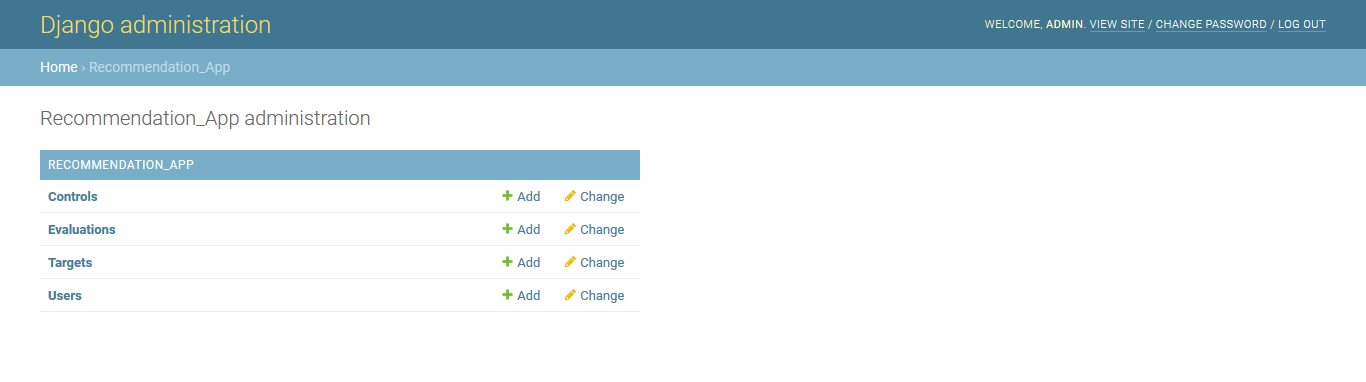
\includegraphics[scale=0.3]{images/MCRS_adminpage.png}
    \caption{Admin page creata automaticamente da Django.}
    \label{fig:MCRS_adminpage}
\end{figure}
%
\begin{figure}[ht!]
    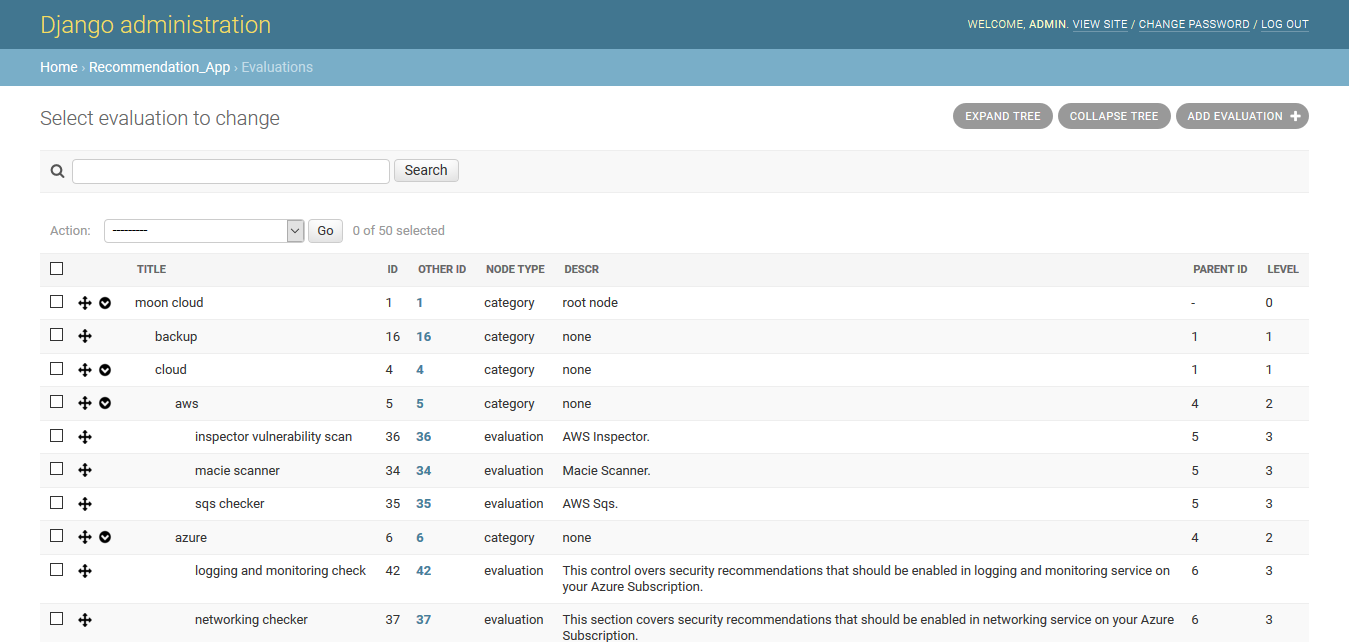
\includegraphics[scale=0.3]{images/MCRS_adminpage_evaluationEX.png}
    \caption{Esempio di Admin page per la tabella delle Evaluation.}
    \label{fig:MCRS_adminpage_evaluationEX}
\end{figure}
%
\begin{figure}[ht!]
    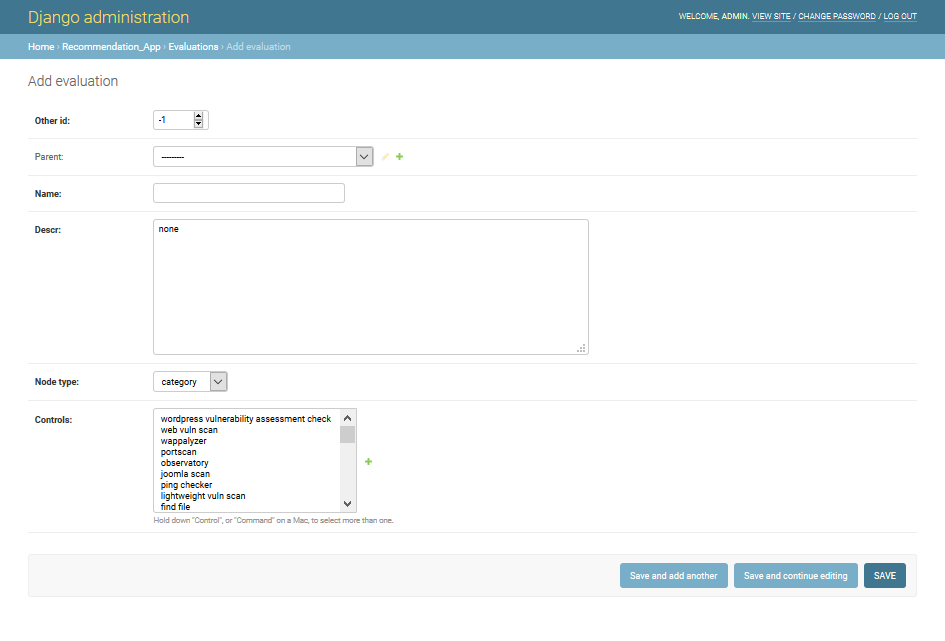
\includegraphics[scale=0.55]{images/MCRS_adminpage_evaluationEX_add.png}
    \caption{Esempio di Admin page per il caso in cui si vuole aggiungere una nuova Evaluation.}
    \label{fig:MCRS_adminpage_evaluationEX_add}
\end{figure}
%
\newpage
% VIEW PER MANTERE LA CONSISTENZA COL MIO DATABASE
\section*{Consistenza tra i database}
% parlare di rest_framework, dei serializer, e url
Per fare in modo che il database creato in questo progetto e l'attuale database utilizzato dalla piattaforma di Moon Cloud 
fossero consistenti, quindi le informazioni presenti nell'uno siano identiche a quelle nell'altro, si è 
pensato d'implementare un sistema di API REST.\hfill\break
Nel caso vengano fatte modifiche, aggiunte o cancellazioni di dati relativi a Controlli, Evaluation, Target, User o Target Type 
è possibile richiamare tramite appositi URL, mostrati nel Listing \ref{lst:view_cos_rec_url}, queste funzioni ed eseguire la relativa 
operazione sul database implmentato nella soluzione, senza dover accedere e manipolare direttamente la base di dati.
\lstset{style=python_code_style}
\begin{lstlisting}[language=Python, label=lst:view_cos_rec_url, caption={Porzione di codice dell'URL Mapper contenti le URL usate per 
    mantenere la consistenza dei dati.}]
# API REST EXTERNAL to maintain database consistency
# Control views
url(r'^control/$', control_views.ControlListCreate.as_view(),
    name="control_list_create_view"),
url(r'^control/(?P<other_id>[0-9]+)/$', control_views.ControlRetrieveDeleteUpdate.as_view(),
    name="control_retrieve_delete_update_view"),
 
# Evaluation views
url(r'^evaluation/$', evaluation_views.EvaluationListCreate.as_view(),
    name="evaluation_list_create_view"),
url(r'^evaluation/(?P<other_id>[0-9]+)/$', evaluation_views.EvaluationRetrieveDeleteUpdate.as_view(),
    name="evaluation_retrieve_delete_update_view"),
 
# Target views
url(r'^target/$', target_views.TargetListCreate.as_view(),
    name="target_list_create_view"),
url(r'^target/(?P<other_id>[0-9]+)/$', target_views.TargetRetrieveDelete.as_view(),
    name="target_retrieve_delete_view"),
 
# User views
url(r'^user/$', user_views.UserListCreate.as_view(),
    name="user_list_create_view"),
url(r'^user/(?P<other_id>[0-9]+)/$', user_views.UserRetrieveDeleteUpdate.as_view(),
    name="user_retrieve_delete_update_view"),
url(r'^user_evaluations/$', user_views.UserEvaluationUpdate.as_view(),
    name="user_evaluations_update_view"),
\end{lstlisting}
%
% IMPLEMENTAZIONE CON DOCKER
\section*{Implementazione in Docker}
Una volta preparata la base e gli algoritmi di raccomandazione, con tutto ciò a essi collegati (View, URL, API REST); l'ultima fase nel ciclo di sviluppo è il 
deployment e la sua preparazione. In questo caso l'app viene deployata, come il resto dei componenti di Moon Cloud, in una serie di Container Docker. Per 
tale ragione, è stato predisposto il file \textit{docker-compose.yml}, il quale viene usato dalla Docker Machine per poter creare un Immagine contenente 
il necessario per l'esecuzione all'interno del Container, oltre alle caratteristiche del Container stesso e delle informazioni usate per poter 
comunicare con l'esterno.
%Codice del dockerfile + SPIEGAZIONE
\lstset{style=python_code_style}
\begin{lstlisting}[language=Xml, label=lst:docker_compose, caption={Contenuto del file docker-compose.yml per il deployment del sistema di raccomandazione 
    all'interno di un Container.}]
    version: '3'

    services:
      db:
        networks:
          - mooncloud
        image: postgres:12.1
        restart: always
        volumes:
          - "./init_db/initdb.sh:/docker-entrypoint-initdb.d/1-initdb.sh"
        environment:
          POSTGRES_USER: postgres
          POSTGRES_PASSWORD: postgres
    
      api:
        networks:
          - mooncloud
        build:
            dockerfile: Dockerfile
            context: .
        command: ./entrypoint.sh
        ports:
          - "8000:8000"
        depends_on:
          - db
        environment:
          DATABASE_HOST: db
          DATABASE_PORT: 5432
          DATABASE_USER: postgres
          DATABASE_PASSWORD: postgres
          DATABASE_NAME: mooncloud_rec
    
    networks:
      mooncloud:
        external: true
\end{lstlisting}
%
Questo file permette di configurare i servizi della propria applicazione; i quali, attraverso un singolo comando, possono essere creati e inizializzati a 
partire da questo singolo file.
La prima riga specifica sempre la versione (\textit{version}) del formato del file di Compose, successivamente si definiscono i \textit{services} e 
le \textit{networks}. In questo progetto si è fatto uso di due servizi (\textit{db} e \textit{api}), i quali speficiano le 
proprietà dei rispettivi Container uno per implementare il database (\textit{db}) e il secondo per le API REST (\textit{api}); nel primo caso per il 
processo di \textit{build} si fa uso di un'Immagine che è già stata pubblicata in un Docker Registry, mentre nel secondo caso essa viene costruita 
a partire dal codice sorgente scritto nel suo \textit{Dockerfile}. Per fare in modo che servizi siano accessibili dall'esterno il numero di porta 
(\textit{ports}) deve essere indicato, nel caso del sevizio \textit{api} ciò è specificato all'interno del \textit{Dockerfile}.\hfill\break
Le \textit{networks} definiscono le regole di comunicazione tra i Container, e tra i Container e gli host; delle reti in comune 
permettono a diversi servizi di essere visibili l'uno con l'altro.
%
\vspace{1.5 cm}
\hfill\break
Ogni qualvolta è stata portata a termine una fase dell'implementazione, proposta in questa tesi, sono state predisposte 
dei processi di verifica del funzionamento del codice scritto fino a quel momento. Questo genere di test, vennero fatti 
per essere certi che le varie fasi fossero in grado di funzionare insieme.\hfill\break
I primi test sono fatti sul database, accertandosi del suo funzionamento e di quello del package MPTT usato 
per costruire la tassonomia delle Evaluation e quella dei Controlli. Successivamente vennero fatte delle verifiche sulla 
corretta interazione, con la base di dati, attraverso le View a scopo didattico e che le modifiche fatte alle admin page 
standard di Django dessero i risultati attesi. Una volta implementati gli algoritmi di raccomandazione, e relative View, 
e il sistema di API REST per il mantenimento della consistenza tra il database, creato in questa soluzione, e quello 
attualmente in uso su Moon Cloud, venne creato un sistema di test automatizzato, grazie alle funzioni built-in di Django, 
in cui ogni test richiama la funzione da testare, salva il suo risultato, e lo confronta con quello atteso, 
oltre a verificare che il codice della risposta HTTP corrisponda a quello atteso.\hfill\break
Per semplificare lo sviluppo e la verifica del corretto funzionamento si è voluto creare dei test aggiuntivi tramite 
l'ausilio di Postman; una piattaforma nata per lo sviluppo e il test di API, inoltre semplifica molti step per il loro 
sviluppo così da poter creare API migliori e più velocemente. Inoltre permette di generare una documentazione 
machine-readable così da rendere le API più facili da usare.

%Durante la scrittura delle View e delle altre parti del codice, sono stati definiti dei test per poter garantire il funzionamento di queste 
%funzioni, anche nel caso di eventuali modifiche successive; questo grazie ai metodi già forniti da Django e all'ausilio di Postman.